\section[Theory]{Theory \textnormal{\cite{GrossMarx+2022}}}
\label{sec:theory}

In the description of condensed matter, tools from classical thermodynamics and statistical physics as well
as quantum mechanical considerations need to be applied. Throughout the following paragraphs, we explore some
of the more well known models in the subfield of thermal properties, specifically for the explanation of the
heat capacity in solids.

\subsection{Heat Capacity}

The heat capacity of any material is defined via
\begin{equation*}
	C \equiv \pfrac{\up{\Delta}Q}{\up{\Delta}T\:}
\end{equation*}
as the amount of heat $\up{\Delta}Q$ corresponding to a unit change $\up{\Delta}T$ in temperature. This is
clearly dependent on the amount of matter, so to allow for comparisons between different materials we can
normalize with volume $V$ or mass $M$ to obtain a specific heat capacity.

\subsubsection{Molar Heat}

In our case, we are interested in the heat capacity per number of particles making up a sample. This leads to
\begin{equation*}
	c \equiv \pfrac{\up{\Delta}Q}{n\up{\Delta}T\:}
\end{equation*}
for the molar heat capacity, where $n$ is the number of \unit{\mole} contained in the substance. To determine
$n$ one can use readily available values of the molar mass $m$ or molar volume $v$ for the given
experimental parameters.

\subsubsection{Measurement}

During the measuring process, it is necessary to constrain certain parameters. To grasp the following relations,
we examine the first and second laws of thermodynamics
\begin{equation*}
	\up{d} U = \up{\delta} Q - \up{\delta} W = T \up{d} S - P \up{d} V
\end{equation*}
where $U$ is the internal energy, $Q$ and $W$ are heat and work, $T$ stands for temperature, $S$ for entropy,
$P$ for pressure and $V$ for volume. The symbols $\up{d}$ and $\up{\delta}$ denote exact and inexact differentials,
respectively. \newpage

From this relation, we identify $\up{\delta} Q = T \up{d} S$ and thereby
\begin{equation*}
	C = T \: \pfrac{\del S}{\del T\:}
\end{equation*}
when translating the defining statement to infinitesimal notation.

\paragraph{Isochoric Case}

At fixed volume, all units of heat result in temperature changes exclusively. The isochoric heat capacity can be written as
\begin{equation*}
	C_V = T \left.\pfrac{\del S}{\del T\:}\right|_V
\end{equation*}
and constitutes an interesting quantity to study the behaviour of materials due to the isolation of otherwise connected effects.

\paragraph{Isobaric Case}

When the pressure is kept constant instead, some of the heat exchange also results in expansion or contraction of the
sample and therefore reduces the total temperature difference. Intuition therefore tells us that $C_P > C_V$ where we write
\begin{equation*}
	C_P = T \left.\pfrac{\del S}{\del T\:}\right|_P
\end{equation*}
for the isobaric heat capacity. This situation is more easily realizable in experiments but comes at the cost of no longer
separating different mechanisms affecting the substance.

\paragraph{Connection}

In order to convert between $C_P$ and $C_V$ we need some generally applicable relationship between the two quantities.
We establish the differential form for entropy
\begin{equation*}
	\up{d}S = \left.\pfrac{\del S}{\del T\:}\right|_V \!\up{d}T + \left.\pfrac{\del S}{\del V\:}\right|_T \!\up{d}V
\end{equation*}
in terms of volume as an extensive and temperature as an intensive property. We obtain
\begin{equation*}
	\left.\pfrac{\del S}{\del T\:}\right|_P \!= \left.\pfrac{\del S}{\del T\:}\right|_V \!+
	\left.\pfrac{\del S}{\del V\:}\right|_T \left.\pfrac{\del V}{\del T\:}\right|_P
\end{equation*}
by differentiating, allowing us to reformulate our desired quantites
\begin{equation*}
	C_P - C_V = T\left(\left.\pfrac{\del S}{\del T\:}\right|_P \!- \left.\pfrac{\del S}{\del T\:}\right|_V \:\right) =
	T\left.\pfrac{\del S}{\del V\:}\right|_T \left.\pfrac{\del V}{\del T\:}\right|_P
\end{equation*}
as the difference between them. \newpage

A combination of Jacobian coordinate transformations and Maxwell relations yields
\begin{equation*}
	C_P - C_V = \alpha_V^2 \, \kappa_T \, TV
\end{equation*}
with the isothermal bulk modulus
\begin{equation*}
	\kappa_T = -V\left.\pfrac{\del P\:}{\del V\:}\right|_T
\end{equation*}
and the volumetric thermal expansion coefficient
\begin{equation*}
	\alpha_V \, = \pfrac{1}{V\:} \left.\pfrac{\del V\:}{\del T\:}\right|_P
\end{equation*}
of the material. For isotropic materials, the last term is equivalent to the form $\alpha_V \, = 3\,\alpha_{\!L}$ via the
linear analogue
\begin{equation*}
	\alpha_{\!L} = \pfrac{1}{L\:} \left.\pfrac{\del L\:}{\del T\:}\right|_P
\end{equation*}
which gives
\begin{equation*}
	C_P - C_V = 9 \, \alpha_{\!L}^2 \, \kappa_T \, TV
\end{equation*}
as the final expression. For typical solids with strong binding forces this difference is negligible, though it becomes
more relevant for liquid or gaseous states of matter.

\subsection{Models}

All approaches discussed in this section model condensed matter as perfect crystal lattices with normal modes of
participating members as purely harmonic oscillations. In the Hooke regime, the center of mass does not change
with increasing or decreasing energy. Accordingly, the volume is constant under heat exchange and the condition
$C_V = C_P$ is always fulfilled. This is of course unphysical, but it should serve as a decent approximation for
the materials we are interested in. To account for thermal contraction, we would need to consider anharmonic
effects by expanding the assumed potential minimum to higher orders.

\subsubsection{Classical Physics}

The equipartition theorem from classical thermodynamics affords a mean energy
\begin{equation*}
	\left< u \right> = \pfrac{1}{2} k_B T
\end{equation*}
to each available degree of freedom. For a singular uncoupled harmonic oscillator, we have the spacial components of
position and velocity as free coordinates. In this view, a three dimensional system of $N$ atoms has an internal energy
\begin{equation*}
	U = 3 N k_B T = 3 nRT
\end{equation*}
when we impose zero equilibrium potential. Here $R = N_{\! A} k_B$ is the universal gas constant, $N_{\! A}$ is the Avogadro
constant and $k_B$ is the Boltzmann constant. \newpage

Because $\up{d}V = 0$ and therefore $\up{d}U = \up{\delta}Q$ we can simply write
\begin{equation*}
	C = \pfrac{\del U}{\del T\:} = 3N k_B = 3nR
\end{equation*}
to find the heat capacity as predicted through the empirical law by Dulong and Petit.

\subsubsection{Quantum Mechanics}

The classical result estimates the heat capacity reasonably well for high temperatures. At lower temperatures however, we
expect quantum mechanical effects to play a significant role. This is explained by the quantization of energy in multiples
of $\hbar\omega$ dividing the range of allowed states into discrete levels. At temperatures where $k_B T \gg \hbar\omega$
the energy space appears continuous to thermal excitations whereas $k_BT \ll \hbar\omega$ forces most members to remain
frozen in the ground state. To visualize this description, figure \ref{fig:quantization} presents a coneptual sketch.

\begin{figure}
	\centering
	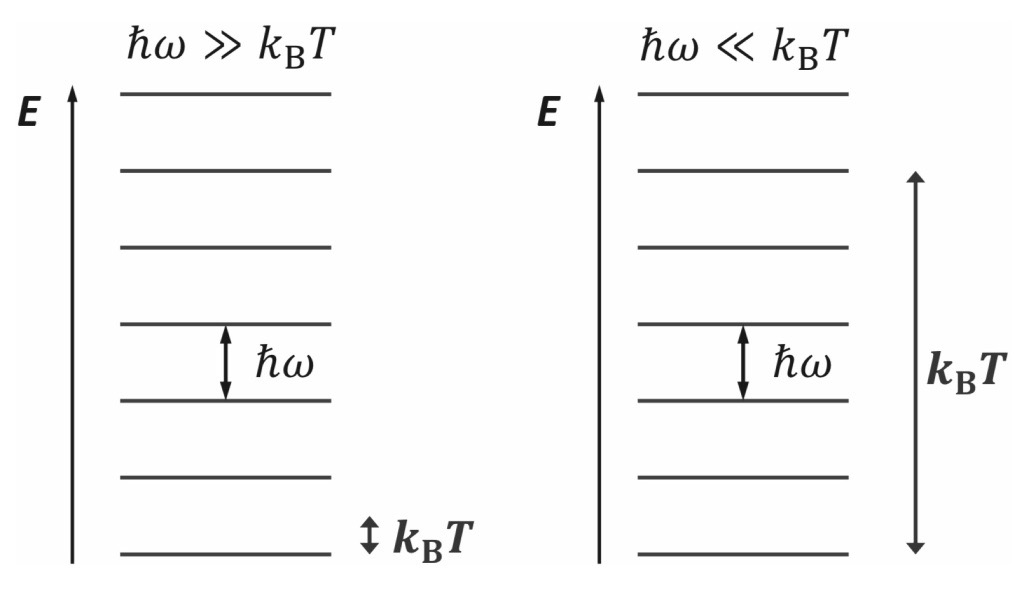
\includegraphics[width=0.4\linewidth]{content/graphics/quantization.jpg}
	\caption{Exemplary energy discretization in low and high temperature limits. \cite{GrossMarx+2022}}
	\label{fig:quantization}
\end{figure}

\paragraph{Phonons}

\begin{figure}
	\centering
	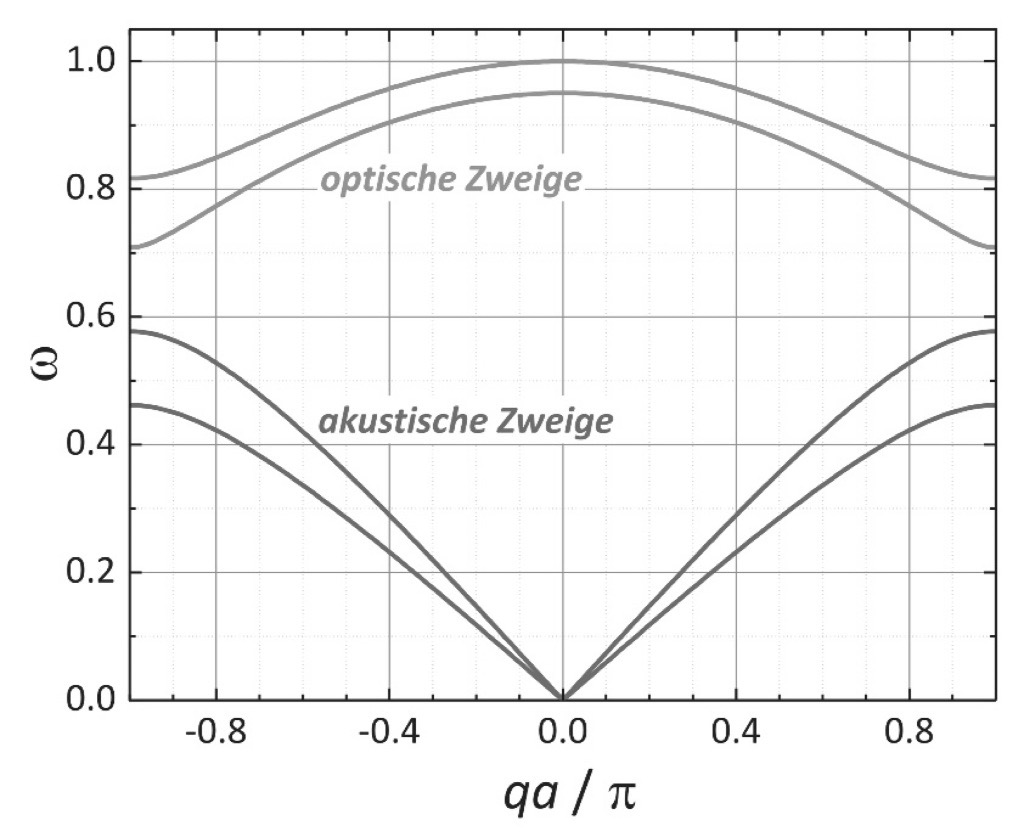
\includegraphics[width=0.45\linewidth]{content/graphics/branches.jpg}
	\caption{Schematic phonon branches inside the first Brillouin zone. \cite{GrossMarx+2022}}
	\label{fig:branches}
\end{figure}


\paragraph{Einstein}

\paragraph{Debye}

\paragraph{Electrons}
